Digital cellular networks are designed to carry many simultaneous conversations across a limited radio spectrum. Each call consists of two independent data streams — one uplink, one downlink — connecting handset and base station. These streams must be separated both by directionality and from the traffic of other users occupying the same band.

Two structural constraints govern how a cellular system organizes radio traffic: duplexing and multiplexing. Duplexing separates the uplink (phone to tower) from the downlink (tower to phone). In frequency division duplexing (FDD), each direction is assigned its own frequency band, allowing simultaneous transmission and reception. In time division duplexing (TDD), both directions share a common band but alternate in fixed, synchronized time slots.

Multiplexing separates users sharing the same physical channel. In frequency division multiple access (FDMA), the spectrum is divided into separate frequency bands, each assigned to a different user. This isolates signals but requires fixed bandwidth allocation and limits how flexibly users can be added or removed. In time division multiple access (TDMA), users transmit in alternating time slots within a repeating frame structure. Each user has exclusive access to the channel during its assigned slot. This improves spectral efficiency, but requires strict global timing to keep transmissions aligned. In code division multiple access (CDMA), all users transmit simultaneously over the same frequency band, but each encodes its data using a unique pseudorandom spreading code. The receiver uses correlation to extract the intended signal. This allows full-time transmission with statistical multiplexing, but demands complex signal separation.

Each multiplexing scheme divides the shared medium along a different axis — frequency, time, or code — but all enforce strict structural requirements on the transmitted signal. In FDMA, users are isolated by frequency: each occupies a separate sub-band, like callers speaking in different rooms. In TDMA, users are separated by timing: they take turns within a shared frame, like speakers passing a microphone in tightly scheduled intervals. In CDMA, all users transmit simultaneously, but each encodes their signal with a distinct pseudorandom code, like voices speaking different languages that can be separated by a trained listener. Despite their differences, all three approaches require that each user’s transmission be confined to a fixed envelope — a burst — with predictable alignment and duration.

These requirements propagate upward through the entire transmission stack. Each burst must arrive in its designated slot, with precisely constrained size and timing. Modulation, equalization, and error correction depend on this regularity. As a result, every upstream layer — from speech encoding to encryption — must preserve the burst structure exactly. The system allows no expansion, delay, or variability. No stage may disrupt length or schedule without undermining synchronization at the physical layer. What is transmitted must be shaped in advance to fit. What is encrypted must already conform.

To transmit speech, the analog signal is sampled at regular intervals and each sample is encoded as a digital number. This raw bitstream is then compressed using a speech codec — a specialized algorithm that reduces bandwidth by representing only perceptually important features. As a toy example, consider a 20 ms segment of audio. Uncompressed, this might require over 2,000 bits. A codec might instead describe it using only pitch, volume, and phoneme class, reducing the bitrate by an order of magnitude.

GSM — the Global System for Mobile Communications — was developed as a pan-European standard for digital cellular networks in the early 1990s. It replaced earlier analog systems with a structured, time-synchronized digital stack designed for interoperability, moderate confidentiality, and efficient spectrum use. The GSM radio interface is based on TDMA: each 200 kHz carrier is divided into repeating time frames of eight slots, with each user assigned one slot per frame. Each slot — or burst — carries 114 bits of payload, framed by synchronization and guard bits.

Voice is transmitted as a sequence of such bursts. Every 20 milliseconds of speech is compressed into a 260-bit frame. These bits are divided into classes by perceptual importance. The most critical will later be protected with more redundancy. Each frame is processed independently and must be transmitted in order, aligned to the caller’s assigned slot. From this point forward, it is treated as a fixed-length atomic unit — encoded, encrypted, and modulated as a whole.

Before transmission, the frame is convolutionally encoded. This adds structured redundancy by producing each output bit as a function of the current and previous inputs. The goal is to enable error correction at the receiver without retransmission. After encoding, the output is interleaved — reordered across time so that localized bit corruption does not overwhelm any one frame. These operations are deterministic and standardized. Their result is a longer, structured bitstream with predictable relationships between positions.

At this point, the data must be encrypted — but without affecting its size or timing. Each burst has a fixed payload size, and must be transmitted precisely at its assigned interval. This rules out block ciphers that expand input or require buffering. The encryption must operate in-place. GSM therefore uses a stream cipher: a keystream is generated and XORed with the data bit-for-bit, producing ciphertext of equal length and immediate readiness for modulation.

GSM fixes the processing order as: compression $\rightarrow$ error correction $\rightarrow$ interleaving $\rightarrow$ encryption. This sequencing reflects a deliberate engineering decision. By placing encryption at the end of the stack, the system isolates cryptographic logic from earlier processing stages. Each module performs a self-contained transformation. This design simplifies implementation but introduces a structural vulnerability.

By the time the bitstream reaches the cipher, it is no longer raw data. It has been processed into a rigid format defined by protocol constraints. This includes:

\begin{itemize}
  \item \textbf{Training sequences} — fixed bit patterns at known positions for synchronization.
  \item \textbf{Padding fields} — deterministic bits inserted to fill incomplete payloads.
  \item \textbf{Error-correction codes} — parity bits computed from public polynomials.
  \item \textbf{Interleaving} — a known permutation applied identically to each block.
\end{itemize}

The structure of GSM messages at the physical layer is rigid by specification. Each 114-bit burst contains payload data bracketed by synchronization and guard intervals of fixed length. Within the payload, the bitstream is heavily preprocessed prior to encryption. Bit patterns associated with training sequences, tail bits, and error-correction codes are defined explicitly by the standard and are identical across sessions. The plaintext entering the encryption algorithm is therefore not random, nor even variable in many locations. It is drawn from a constrained distribution with high predictability and low entropy in fixed subregions. A passive observer capturing encrypted GSM traffic does not face an opaque binary stream; instead, they receive ciphertext derived from partially labeled inputs whose positions and formats are specified in advance by protocol structure.

This situation is made worse by the ordering of operations in the transmission pipeline. Speech data is first compressed using a perceptual codec, then passed through a convolutional encoder that adds structured redundancy. The encoded bitstream is then interleaved across time to improve resistance to burst noise. These transformations are deterministic and public. No secret state is introduced prior to encryption. Each operation adds statistical regularity or linear dependence, which survives intact through the encryption process. GSM uses a stream cipher that encrypts each bit independently using a keystream XOR. As a result, the cipher preserves structure in a way that a block cipher with diffusion would not. Linear relations introduced by coding are reflected in the ciphertext. Bit positions with predictable values retain that predictability post-encryption. Every preprocessing step compounds the amount of accessible structure exposed to a passive observer.

This deterministic exposure allows the ciphertext itself to leak constraints on the keystream. Suppose the channel coding step introduces a parity check — a known XOR relation among data bits. Because encryption is bitwise, the corresponding ciphertext bits satisfy the same parity relation among their respective keystream values. An attacker does not need to know the underlying data to deduce this constraint. By collecting multiple ciphertext samples, each reflecting similar structural patterns but different realizations of the keystream, the attacker can build a system of equations that gradually reduces the candidate key space. In the case of GSM, voice frames are transmitted redundantly across multiple bursts, increasing the number of observable ciphertext instances derived from aligned inputs. Repeated encipherment of similar structure with the same key transforms the keystream into an object of analysis rather than protection.

This vulnerability was exploited explicitly in the work of Eli Biham, Elad Barkan, and Nathan Keller. In 2003, they demonstrated a ciphertext-only attack against A5/2 capable of recovering the full 64-bit session key in under one second, using only milliseconds of intercepted communication. The attack made no assumptions about plaintext content beyond its adherence to GSM’s structural format. The weakness was not due to the cipher’s internal design alone. It was the result of applying error correction and interleaving before encryption, allowing algebraic methods to exploit the resulting regularity. The attack avoided brute-force enumeration entirely. Instead, it reduced the key recovery problem to solving a sparse system of equations derived from keystream parity constraints — a task tractable on standard computing hardware.

In the same year, the authors presented an active attack that used this weakness in A5/2 to compromise A5/1. GSM allows the base station to select the cipher for communication. A rogue station can impersonate a valid tower and request a downgrade to A5/2 from a handset that supports it. Once the device complies, the attacker captures the A5/2-encrypted exchange, recovers the session key, and then uses that key to decrypt subsequent bursts sent using A5/1. This is possible because GSM reuses the session key across ciphers during a session. The presence of A5/2 in the cipher suite thus undermines A5/1, regardless of whether the latter is ever explicitly requested by the attacker. Any device that implements A5/2 inherits its vulnerabilities and propagates them to the stronger cipher via shared key state.

Barkan and Biham continued to refine their attacks. In 2005, they improved known-plaintext techniques against A5/1, specifically targeting its irregular initialization procedure. This reduced the computational burden of recovering internal state, particularly in scenarios with limited plaintext exposure. However, their most significant advance came in 2006, when they extended ciphertext-only techniques to A5/1 itself. The approach required far more ciphertext and offline preprocessing than the attack on A5/2, but the principle was similar. By leveraging the publicly known convolutional codes used before encryption, the attackers extracted algebraic relations between ciphertext bits and the keystream. These relations were then used to filter candidate internal states of the cipher’s LFSRs, narrowing the search space to feasible dimensions. The complexity of the attack remained high, but it fell within the capabilities of a moderately resourced organization with access to terabyte-scale storage and standard computational infrastructure.

The attack on A5/1 demonstrated that GSM’s vulnerability was not confined to a single algorithm. It emerged from the interplay between encryption placement, channel structure, and cipher reuse. GSM’s architectural decision to support multiple ciphers without enforcing mutual isolation of key state allowed one weak algorithm to compromise the integrity of the entire suite. Because GSM does not authenticate base stations, handsets cannot verify that cipher selection is legitimate. Any device supporting A5/2 remains exposed to downgrade. Once the session key is recovered through a break of A5/2 — whether using algebraic decoding or parity-based keystream reconstruction — that same key grants access to A5/1-protected content. GSM’s cipher suite is therefore not modular. Its effective security is bounded not by the strongest cipher in use, but by the weakest that is supported. A5/2’s inclusion rendered A5/1 susceptible by transitive failure. The critical flaw was not merely that A5/2 was insecure, but that GSM allowed its presence to affect unrelated cryptographic layers.


\begin{commentary}[Protocol Assumptions and Personal Entry Point]

The weakest points in deployed cryptographic systems are rarely in the mathematics. They are in the layers that surround it: in protocol assumptions, state handling, framing conventions, or timing logic. This is why cryptographic standards are slow to change — not because better ciphers are unavailable, but because known, tested flaws are often safer than untested replacements. The defensive posture of a system is not just algorithmic strength, but mostly accumulated knowledge of how it fails.

I first encountered this issue in a lecture by Eli Biham around 2003. He outlined the GSM vulnerability using nothing but XOR equations, known plaintext segments, and short recurrence relations. For once, the attack did not require knowing the full formalism of block cipher construction or number theory. It showed that security could collapse under structural exposure — and that the analysis of “where” in a system encryption occurs mattered as much as “how.”
\end{commentary}

\thispagestyle{empty}
\begin{figure}[p]
\centering
\fbox{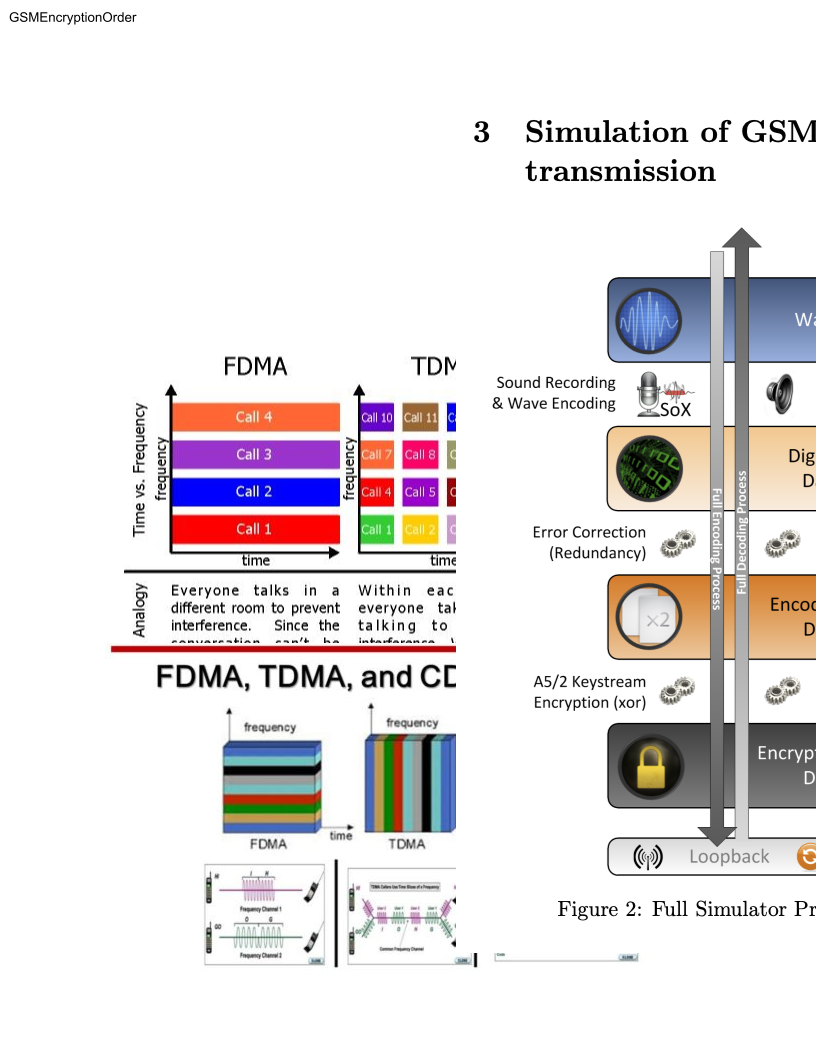
\includegraphics[width=\textwidth,height=\textheight,keepaspectratio]{12_GSMEncryptionOrder/DMA_illu.png}}
\end{figure}

